\documentclass[UTF8]{ctexart}
%宏包:
\usepackage{abstract}
\usepackage{lettrine}
\usepackage{multicol}
\usepackage{cite}
\usepackage{mathtools}
\usepackage{graphicx}
\usepackage{subfigure}
\usepackage{caption}
\usepackage{booktabs}
\usepackage{multirow}
\usepackage{diagbox}
\usepackage{makecell}
\usepackage{placeins}
\usepackage{float}
\usepackage{geometry}
\usepackage{amssymb}
\usepackage{xcolor}
\usepackage{soul}
\usepackage{rotating}
\usepackage{hyperref}
%\pagecolor[rgb]{0.1, 0.1, 0.1}
%\pagecolor[rgb]{0.4, 0.4, 0.4}
%\pagecolor{black} 
%\definecolor{Firebrick4}{RGB}{255, 255, 255}
%\definecolor{shadecolor}{rgb}{0.92,0.92,0.92}

%\textcolor[rgb]{1,0,0}{text}

%\textcolor{red/blue/green/black/white/cyan/magenta/yellow}{text}

%没有缩进           \noindent
%粗体,放大         {\bf\large 12}:12
%另段:           空行
%空行另段:      \\+空行
%文内插入公式如  $F_s=m_sa$
%单行插入公式   \begin{equation}
%               \end{equation}
%              \begin{displaymath}
%             \end{displaymath}
%乘号         \times
%分号         \frac{a}{b}
%绝对值      \left|a \right|
%根号        \sqrt{a}
%            \sqrt[3]{0}
%大于等于     \geq 0
%小于等于     \leq 0
%不等于        \ne 0   (b\ne 0)
%k属于R      a> 0,($k \in R $)
%集合   N:非负整数集合或自然数集合du{0,1,2,3,…}
%       Z:整数集合zhi{…,-1,0,1,…}
%       Q:有理数集合
%       R:实数集合(包括有理数和无理数)

%       R+:正实数集合
%       R-:负实数集合
%       C:复数集合
%       ∅ :空集(不含有任何元素的集合)
%       N*或N+:正整数集合{1,2,3,…}
%       Q+:正有理数集合
%       Q-:负有理数集合
%       省略号就用\cdots了
%      求和要加\displaystyle
%空格    \qquad 

\begin{document}
	
	%\markright{页眉}

%封面
\title{系数阵笔记1.5}
\author{浩于长空}

%\date{}

\maketitle

$$\text { Show that if } a, b, c,\geq 0,(a b+b c+c a)\left(\frac{1}{(a+b)^{2}}+\frac{1}{(b+c)^{2}}+\frac{1}{(c+a)^{2}}\right) \geq \frac{9}{4}
$$
\begin{flushright}
	\text { (Crux Problem No.1940 \& Iran TST,1996) }
\end{flushright}
\begin{displaymath}
\end{displaymath}

\begin{center}
	\href{https://github.com/Raymond0Hui/LaTeXwork-open}{开源于GitHub}
\end{center}

%摘要
\begin{abstract}
	有关三元齐次不等式的小讲堂的笔记,不会对高考或竞赛很有用……大家看心情看
	这里很多内容会很抽象很玄学,而且这个技术更像心法,未必能把自己的思考完全传达出来,能不能听懂全靠缘分,能保证的是Iran96这种简单的不等式以后遇到轻松解决。
\end{abstract}

\newpage

$$ (\displaystyle \sum xy)(\displaystyle \sum \dfrac{1}{(x+y)^{2}})\geq \dfrac{9}{4}$$
$$\Leftrightarrow 
4(\displaystyle \sum xy)(\displaystyle \sum (y+z)^{2}(z+x)^{2})\geq 9\prod (x+y)^{2}$$
$$\Leftrightarrow 
4\left[
\begin{smallmatrix}
	0& &1& &0\\
	&1& &1&\\
	& &0& &\\
\end{smallmatrix}
\right]
\left[\displaystyle \sum 
\begin{smallmatrix}
	0& &0& &1& &0& &0\\
	&0& &2& &2& &0&\\
	& &0& &4& &0& &\\
	& & &2& &2& & &\\
	& & & &1& & & &\\
\end{smallmatrix}
\right]\geq 9\prod 
\left[
\begin{smallmatrix}
	1& &2& &1\\
	&0& &0&\\
	& &0& &\\
\end{smallmatrix}
\right]
$$
$$\Leftrightarrow 
4\left[
\begin{smallmatrix}
	0& &1& &0\\
	&1& &1&\\
	& &0& &\\
\end{smallmatrix}
\right]
\left[
\begin{smallmatrix}
	1& &2& &3& &2& &1\\
	&2& &8& &8& &2&\\
	& &3& &8& &3& &\\
	& & &2& &2& & &\\
	& & & &1& & & &\\
\end{smallmatrix}
\right]\geq 9
\left[
\begin{smallmatrix}
	0& &0& &1& &2& &1& &0& &0\\
	&0& &2& &6& &6& &2& &0&\\
	& &1& &6& &10& &6& &1& &\\
	& & &2& &6& &6& &2& & &\\
	& & & &1& &2& &1& & & &\\
	& & & & &0& &0& & & & &\\
	& & & & & &0& & & & & &\\
\end{smallmatrix}
\right]$$
$$\Leftrightarrow 
4\left[
\begin{smallmatrix}
	0& &1& &2& &3& &2& &1& &0\\
	&1& &5& &13& &13& &5& &1&\\
	& &2& &13& &24& &13& &2& &\\
	& & &3& &13& &13& &2& & &\\
	& & & &2& &5& &2& & & &\\
	& & & & &1& &1& & & & &\\
	& & & & & &0& & & & & &\\
\end{smallmatrix}
\right]\geq 9
\left[
\begin{smallmatrix}
	0& &0& &1& &2& &1& &0& &0\\
	&0& &2& &6& &6& &2& &0&\\
	& &1& &6& &10& &6& &1& &\\
	& & &2& &6& &6& &2& & &\\
	& & & &1& &2& &1& & & &\\
	& & & & &0& &0& & & & &\\
	& & & & & &0& & & & & &\\
\end{smallmatrix}
\right]
$$
$$\Leftrightarrow 
\left[
\begin{smallmatrix}
	0& &4& &-1& &-6& &-1& &4& &0\\
	&4& &2& &-2& &-2& &2& &4&\\
	& &-1& &-2& &6& &-2& &-1& &\\
	& & &-6& &-2& &-2& &-6& & &\\
	& & & &-1& &2& &-1& & & &\\
	& & & & &4& &4& & & & &\\
	& & & & & &0& & & & & &\\
\end{smallmatrix}
\right]\geq 0
$$
\begin{center}
	
\includegraphics[width=0.25\linewidth]{z}
\end{center}

\newpage
%目录
\tableofcontents

\newpage

\section{预备知识} 
\subsection{杨辉三角}
我们先从杨辉三角说起,姑且默认大家都知道杨辉三角
\subsection{舒尔不等式}
$ a,b,c \geq 0,t\in \mathbb{R}\implies a^{t}(a-b)(a-c)+b^{t}(b-c)(b-a)+c^{t}(c-a)(c-b)\geq 0$\\
证明:由对称性,不妨设$ a\geq b\geq c,则a^{t}-b^{t}+c^{t}\geq 0 $\\
$ a^{t}(a-b)(a-c)+b^{t}(b-c)(b-a)+c^{t}(c-a)(c-b)=a^{t}(a-b)^{2}+(a-b)(a-c)(a^{t}-b^{t}+c^{t})+c^{t}(b-c)^{2}\geq 0 $\\
核心思想就是,把$ a-c $这个大数,拆成$ a-b $和$ b-c $充分利用其非负性\\
像这样的都是schur:\\
$\displaystyle  \sum  a^{m}\left(a^{n}-b^{n}\right)\left(a^{n}-c^{n}\right)$,$\displaystyle \sum b^{m} c^{m}\left(a^{n}-b^{n}\right)\left(a^{n}-c^{n}\right)$\\
当$ t $取$ 0 $时,即$ \displaystyle  \sum a^{2}-\displaystyle  \sum ab\geq 0 $
\subsection{}
我们意图配出$ F=P+Q+R+ $……其中$ P,Q,R $都是已知非负的结构,那么所谓提出一个$ P $就是考察$ F-P $,对$ F-P $继续观察,减去已知非负之后,专注于剩下的问题,比如再发现$ F-P $可以提个$ Q $,就继续考察$ F-P-Q $,当然,发现放过头了就返回上一步。\\

配方法的一个主要想法就是从外往里剥,如果能不断把角上的正项妥善使用,没有放过头的话,问题就会变得越来越容易处理,毕竟随着角一个个变成0,整个阵(指非零项点位构成的凸包)会越来越小。
\section{二元系数组}
\subsection{定义}
我们已经知道了杨辉三角,杨辉三角本身其实就暗示了“一排数字可以和一个二元齐次多项式相对应”。\\
比如$ [1] $对应$ 1 $,$ [1,1] $对应$ a+b $,$ [1,2,1] $对应$ a^{2}+2ab+b^{2} $……依此类推,那么自然地
$$[1,0,2]_{a, b}=a^{2}+2 b^{2}$$
于是我们姑且作这样的记号,$ [1,0,2] $姑且叫做二元系数组
\subsection{二元系数组的运算性质}
下面我们来观察感受一下系数组的运算性质:\\
其实大家学多项式乘法竖式的时候应该对这种运算方式有所了解,比如$ [1,1]$ × $[1,0,0,1]=[1,1,0,1,1] $,这其实可以利用乘法分配律,也就是$ [1,1]$ × $[1,0,0,1]=[1,1]$ × $[1,0,0,0]+[1,1]$ × $[0,0,0,1]=[1,1,0,0,0]+[0,0,0,1,1]=[1,1,0,1,1] $,考虑到他和多项式同构所以系数组可以有分配律,\\
再例如:
$[1,2,3] \times[1,0,1]=[[1,2,3], 0,[1,2,3]]=[1,2,4,2,3]$,或者我们可以这么理解:
\begin{center}
	\begin{tabular}{ccccc}
		&  & 1 & 2 & 3 \\
		1& 2 & 3 &  &  \\
		\hline
		1& 2 & 4 & 2 & 3 \\
	\end{tabular}
\end{center}
$[1,2,3] \times[1,2,3]=[1 \times[1,2,3], 2 \times[1,2,3], 3 \times[1,2,3]]=[1,4,10,12,9]$或者
\begin{center}
	\begin{tabular}{ccccc}
		
		&  & 3 & 6 & 9 \\
		& 2 & 4 & 6 &  \\
		1& 2 & 3 &  &  \\
		\hline
		1& 4 & 10 & 12 & 9 \\
	\end{tabular}
\end{center}
可以发现,这其实就类似多项式的乘法,唯一的区别就是系数组的运算不进位。
\section{系数阵}
\subsection{定义}
把系数组变成三元的,就是系数阵,我们把下面这个东西叫做三元系数阵,设这个东西第一行有$ n+1 $个数,则称它是$ n $阶的。和上面的二元情形类似,它和三元齐次式之间一一对应。左上角的数对应$ a^n $系数,右上角对应$ b^n $系数,下角对应$ c^n $系数,三元齐次式写成这个样子的主要好处就是,使得我们不用写$ a^{3}b^{2}c $之类的东西了,只需要书写系数,这会使得我们更加便于观察一个三元齐次式的结构。

\renewcommand*{\arraystretch}{1.732}\[\left[\begin{matrix}
	x_{00}& & x_{01}& & x_{02} & & \cdots&&  x_{0n}\\
	& x_{10}& & x_{11}& &\cdots&& \begin{sideways}$\ddots$\end{sideways}& \\
	& & x_{20}& &\cdots&& \begin{sideways}$\ddots$\end{sideways}& & \\
	& & & \ddots&& \begin{sideways}$\ddots$\end{sideways} & & & \\
	& & & & x_{n0}& &&& \\
\end{matrix}\right]\]
或者把它倒过来,左下角对应$ a^n $系数,右下角对应$ b^n $系数,上角的数对应$ c^n $系数。
\renewcommand*{\arraystretch}{1.732}\[\left[\begin{matrix}
	& & &&  x_{30}& && & \\
	& & &\begin{sideways}$\ddots$\end{sideways}& & \ddots&& & \\
	& & x_{20}& & \cdots&&\ddots& & \\
	& x_{10}& & x_{11}&&\cdots& & \ddots& \\
	x_{00}& & x_{01}& & x_{02} & &\cdots&& x_{0n}\\
\end{matrix}\right]\]
例如:$ a+b+c= $
\renewcommand*{\arraystretch}{1.732}\[\left[\begin{matrix}
	1& &1 \\
	& 1&\\
\end{matrix}\right]\]

$ a+2b+3c= $
\renewcommand*{\arraystretch}{1.732}\[\left[\begin{matrix}
	1& &2 \\
	& 3& \\
\end{matrix}\right]\]
$ a^{3}+2b^{3}+3a^{2}b+4c^{3}= $
\renewcommand*{\arraystretch}{1.732}\[\left[\begin{matrix}
	1& & 3& & 0& &2 \\
	& 0& &0 & &0 & \\
	& & 0& &0 & & \\
	& & & 4& & & \\
\end{matrix}\right]\]
\subsection{系数阵的运算}

首先要知道的是一个系数阵乘一个单项系数阵的规律,比如系数阵$ 3 $阶乘$ 3 $阶结果是$ 6 $阶。
我们拿一个$ a^{3}b^{2}c $看
 \begin{center}
 	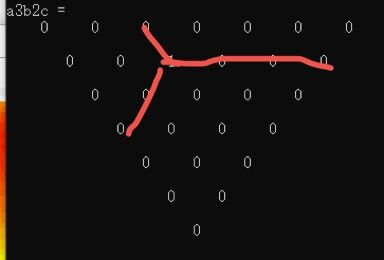
\includegraphics[width=0.36\linewidth]{010}
 \end{center}
你会发现,这个“1”在$ a $角的方向上距离边的距离是$ 3 $,
$ bc $同理,每个数所处的坐标和指数向量是对应的,用的就是齐次坐标的规则。
\begin{center}
	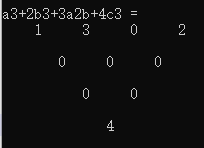
\includegraphics[width=0.25\linewidth]{020}
\end{center}
现在我们把这个东西和刚才那个单项式相乘,大家应该能看出发生了什么
\begin{center}
	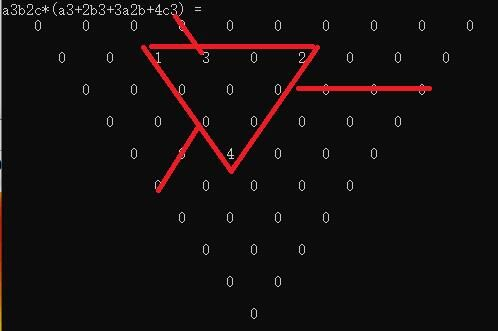
\includegraphics[width=0.4\linewidth]{030}
\end{center}
于是我们来看看这个写法对于三元齐次多项式的乘法带来了怎样一些便利,比方说,三元的杨辉三角现在$ (a+b+c)^{3} $已经有了,我们如何计算$ (a+b+c)^{4} $
\begin{center}
	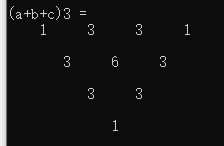
\includegraphics[width=0.3\linewidth]{040}
\end{center}
类似二元系数组,我们可以想象这样的一个感觉,把$ (a+b+c)^{3} $分别乘上$ a,b,c $然后加起来
\begin{center}
	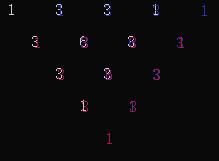
\includegraphics[width=0.3\linewidth]{050}
\end{center}
或者
\begin{center}
	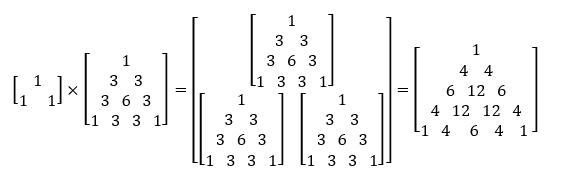
\includegraphics[width=0.6\linewidth]{060}
\end{center}
如果我们直接去思考“最后的这些数由何而来”,就可以这样算出来
\begin{center}
	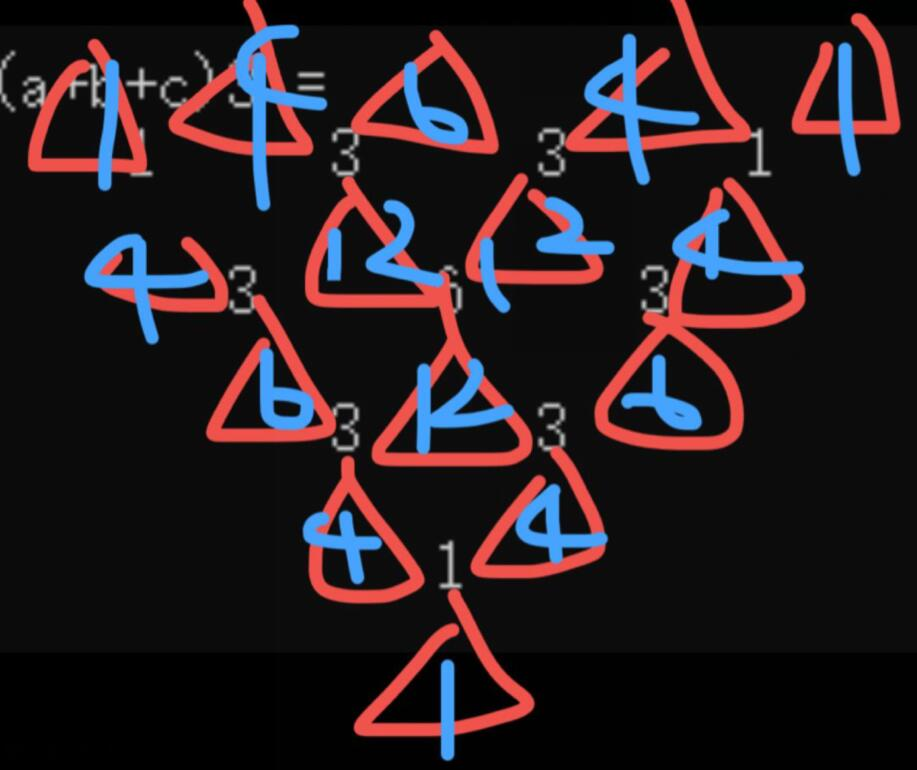
\includegraphics[width=0.27\linewidth]{070}
\end{center}
这也正是杨辉三角的思路在三元情形下的推广,由此我们可以看出,系数阵在“乘以$ (a+b+c) $”这个操作上是带来便利的,此外系数阵还有一个便利,在作轮换和的时候也带来方便。比如说我们把$ (a+b+c)^{3}(a+b+c) $视作$ \displaystyle \sum((a+b+c)^{3}a) $ ,$ (a+b+c)^{3}a $就是
\begin{center}
	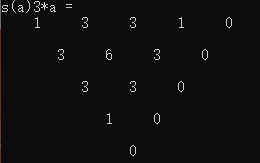
\includegraphics[width=0.31\linewidth]{080}
\end{center}
$ a $角方向加一排$ 0 $,对这个式子作轮换和的话,我们只需要盯着旋转对称的位置相加就行
大体像这个样子,剩下的地方可以直接根据对称性写出来,这里体现的是系数阵在轮换和操作上带来的便利。

\begin{center}
	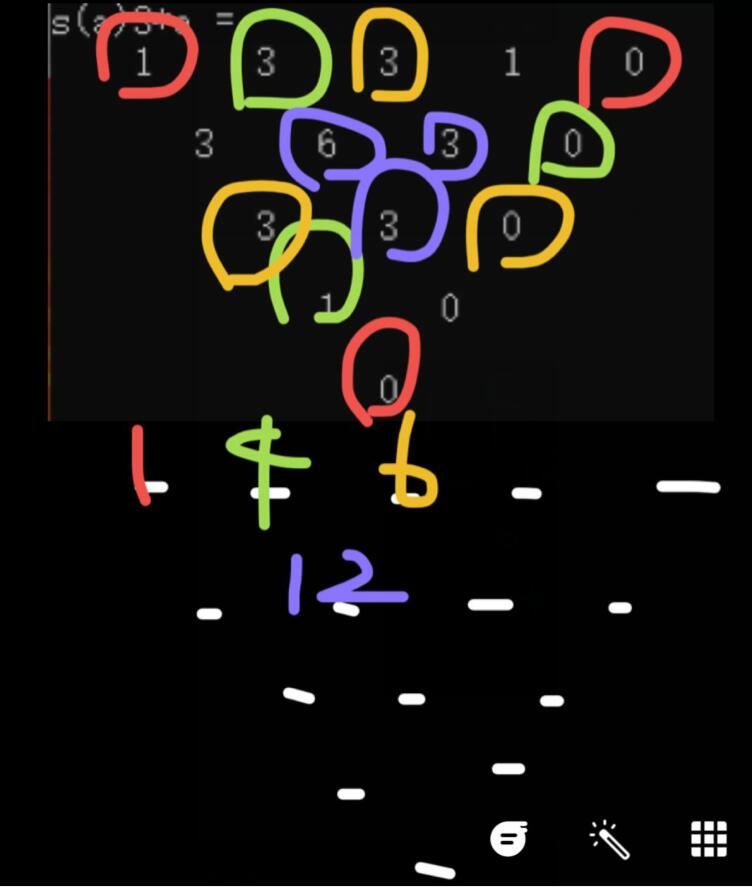
\includegraphics[width=0.35\linewidth]{090}
\end{center}
值得一提的是,如果知道结果是轮换的或轮换对称的,就可以只关注一部分位置上的系数了,此外$ \prod (a-b) $、$ \prod (a+b) $、$ Π(a-b)^{2} $、$ \prod (a+b)^{2} $不难背出来,特别是$ \prod (a-b)^{2} $很有必要背出来,是个很强的结构,记得注意一个多项式被$ a-b $整除的话每行总和都是$ 0 $,对称位置直接写,意思就是不要把整个复制成三份叠起来,这样不好想象,而是去找每一项的来源,这样就可以从被乘的阵上直接读了,乘$ \displaystyle \sum a $、$ \displaystyle \sum ab $、$ \displaystyle \sum a^{2} $之类的都可以用这个技巧,$ a+b $也可以
\subsection{习题}

(1)用系数阵计算$ (a+b)^{2}·(a+c)^{2} $,观察结果形式的特点

(2)如何用系数阵计算$ P(a,b,c)×(ab+ac+bc) $,当然$ P(a,b,c) $齐次

(3)如何用系数阵计算轮换对称和

(4)用系数阵方法将Iran96不等式通分

习题2的话,乘$ (ab+ac+bc) $和乘$ (a+b+c) $差不多,比如要计算这个东西乘$ (ab+ac+bc) $的话,可以在心里画这样一些倒三角求和,蓝色的就是积了。
\begin{center}
	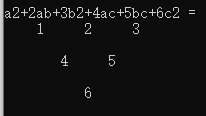
\includegraphics[width=0.35\linewidth]{100}
\end{center}
\begin{center}
	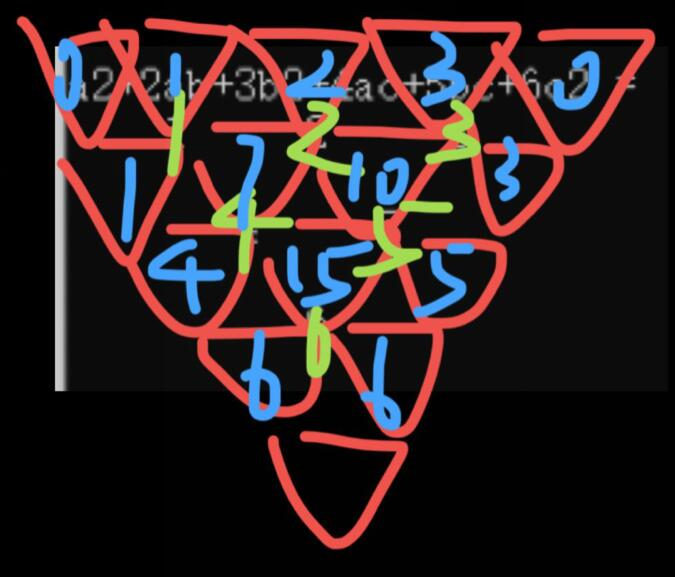
\includegraphics[width=0.35\linewidth]{110}
\end{center}
\section{简单均值不等式}
这里我们只探讨【对于若干系数为1的单项式使用AM-GM不等式】的特点

\subsection{简单的均值不等式}
我们可以先观察几个例子,首先对于$ a^{2}+b^{2}\geq2ab $,即$ a^{2}+b^{2}-2ab\geq0 $

我们知道,$ a^{2}+b^{2}-2ab= $
\renewcommand*{\arraystretch}{1.732}\[\left[\begin{matrix}
	1& & -2& &1 \\
	& 0& &0 & \\
	& & 0& & \\
\end{matrix}\right]\]

$ a^{2}+c^{2}-2ac $的话就是转一下
\renewcommand*{\arraystretch}{1.732}\[\left[\begin{matrix}
	1& & 0& &0 \\
	& -2& &0 & \\
	& & 1& & \\
\end{matrix}\right]\]

那在找个次数高点的例子,$ a^{4}+b^{2}c^{2}-2a^{2}bc= $
\renewcommand*{\arraystretch}{1.732}\[\left[\begin{matrix}
	1& & 0& &0& & 0& &0\\
    & 0& & -2&&0 & & 0&\\
    & & 0& &0& & 1& &\\
    & & & 0&& 0& & &\\
    & & & &0& & & &\\
\end{matrix}\right]\]

到这里其形状的规律已经很明显了,就是“两个1以及其中点处的-2”,实际上根据系数阵的定义很容易验证这一点,
那么再看看三元的情形

$ a^{3}+b^{3}+c^{3}-3abc= $
\renewcommand*{\arraystretch}{1.732}\[\left[\begin{matrix}
	1& & 0& &0& & 1\\
	& 0& & -3& &0 &\\
	& & 0& &0& & \\
	& & & 1& & &\\
\end{matrix}\right]\]

$ a^{2}b+b^{2}c+c^{2}a-3abc= $
\renewcommand*{\arraystretch}{1.732}\[\left[\begin{matrix}
	0& & 1& &0& & 0\\
	& 0& & -3& &1 &\\
	& & 1& &0& & \\
	& & & 0& & &\\
\end{matrix}\right]\]

$ a^{2}b+ab^{2}+c^{3}-3abc= $
\renewcommand*{\arraystretch}{1.732}\[\left[\begin{matrix}
	0& & 1& &1& & 0\\
	& 0& & -3& &0 &\\
	& & 0& &0& & \\
	& & & 1& & &\\
\end{matrix}\right]\]
我们可以惊讶地发现,其形态就是“三个$ 1 $以及其重心处的$ -3 $”,同理$ n $元的情况也是如此,应当是“$ n $个$ 1 $以及其重心处的$ -n $”
那么这里作一个小补——这些$ 1 $可以有部分重合的,比如\\
$ a^{3}+a^{3}+b^{3}-3a^{2}b= $
\renewcommand*{\arraystretch}{1.732}\[\left[\begin{matrix}
	2& & -3& &0& & 1\\
	& 0& & 0& &0 &\\
	& & 0& &0& & \\
	& & & 0& & &\\
\end{matrix}\right]\]

对应的就是重合的两个$ 1 $和另一个$ 1 $与这三点重心上的$ -3 $

这个大家应该不难接受,那么我们来看一个简单的例子吧
$$
\begin{gathered}
	a, b, c \geq 0, \quad \text { 求证: } \sum a^{5}+2 \sum a^{2} b^{2} c \geq 3 \sum a^{3} b c
\end{gathered}
$$
\begin{center}
	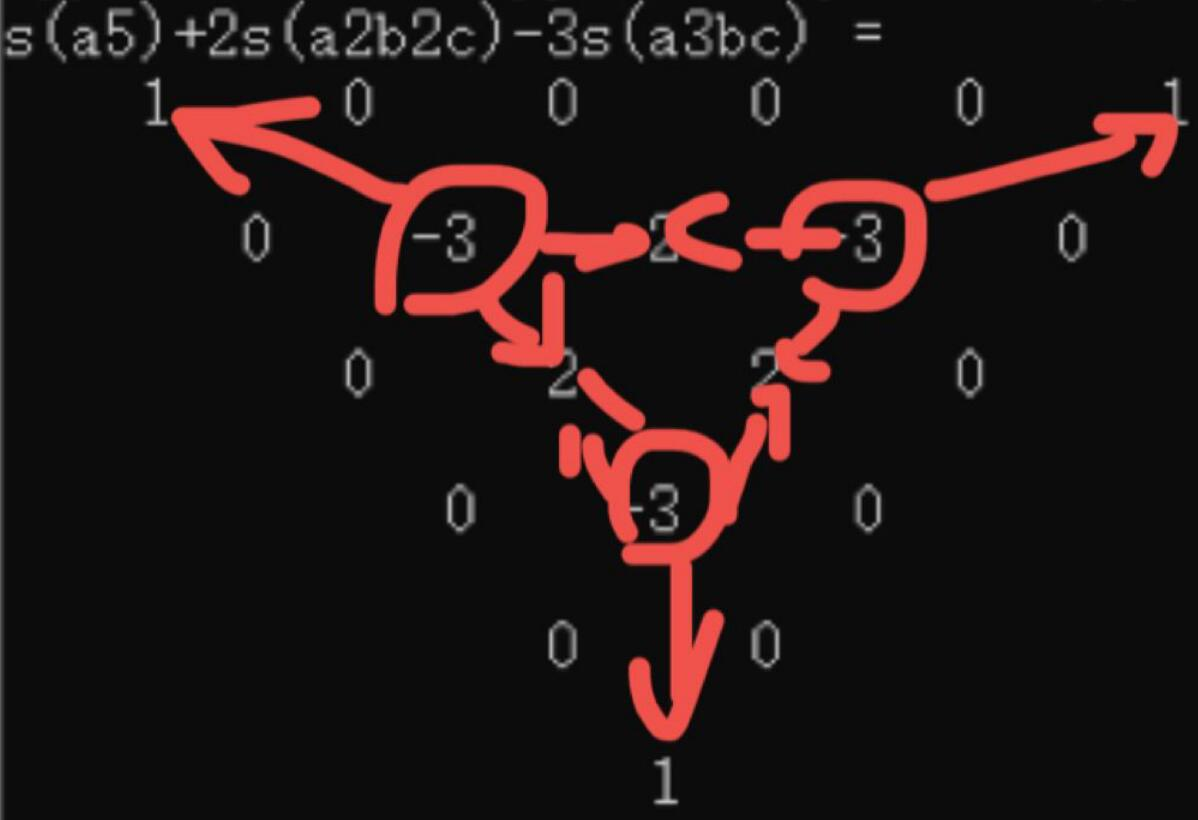
\includegraphics[width=0.4\linewidth]{120}
\end{center}

我们只需看看负项,找找让哪些正项来对付就行,里应外合。下一个例子

$$ a, b, c \geq 0, \quad \text { 求证: } \sum a^{3} b \geq \sum a^{2} b c
$$

接下来我们有两种做法,法一比较容易想到,把它拆成三组$ [1,-2,1] $,每一个$ -1 $拆成$ 1 $和$ -2 $\\
$ \displaystyle \sum (a^{3} b-a^{2} b c)= $
\renewcommand*{\arraystretch}{1.732}\[\left[\begin{matrix}
	0& &1& &0& &0& &0\\
	&0& &-1& &-1& &1&\\
	& &0& &-1& &0& &\\
	& & &1& &0& & &\\
	& & & &0& & & &\\
\end{matrix}\right]\]
换言之也就是:\\
\begin{center}
	注意到$ \displaystyle \sum a^{3} b-\displaystyle \sum a^{2} b c=\displaystyle \sum b c(a-b)^{2} \geq 0 $得证
\end{center}
那么再看一个比较通用的法二
$ \Box a^{3} b+\Box b^{3} c+\Box c^{3} a \geq \Box a^{2} b c $
我们不难想象可以通过均值凑出这样的一个局部,而且我们可以用待定系数法解出来,实际上这个系数是4,1,2,
$ 4a^{3}b+b^{3}c+2c^{3}a-7a^{2}bc= $\\
\renewcommand*{\arraystretch}{1.732}\[\left[\begin{matrix}
	0& &4& &0& &0& &0\\
	& 0& &-7& &0& &1&\\
	& &0& &0& &0& &\\
	& & &2& &0& & &\\
	& & & &0& & & &\\
\end{matrix}\right]\]
那么接下来介绍一下在系数阵里如何快速地凑出这三个数,假定我们还不知道它应该是4,1,2。设之为$ p,q,r $,中间那个自然得是$ -(p+q+r) $,我们要保证的是处于$ a^{3}b $及其轮换位置上的、质量$ p,q,r $的三个质点其质心在$ a^{2}bc $的位置上。这其实就是奔驰定理(或拉密定理)

\begin{center}
	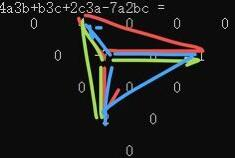
\includegraphics[width=0.4\linewidth]{130}
\end{center}

也就是说这三个系数之比应当等于这三块的面积比,不妨绿色那块面积是1,于是显见红色是2、蓝色是4,这样就直接凑出来啦,这里建议熟悉$ S=\displaystyle \frac{1}{2}ab  \sin \theta $
。事实上,此处也可以结合皮克定理,数“有多少个180°”,如下面这个例子:\\
$ \displaystyle  \sum a^{3} b^{2} \geq \displaystyle  \sum a^{2} b^{2} c $

\begin{center}
	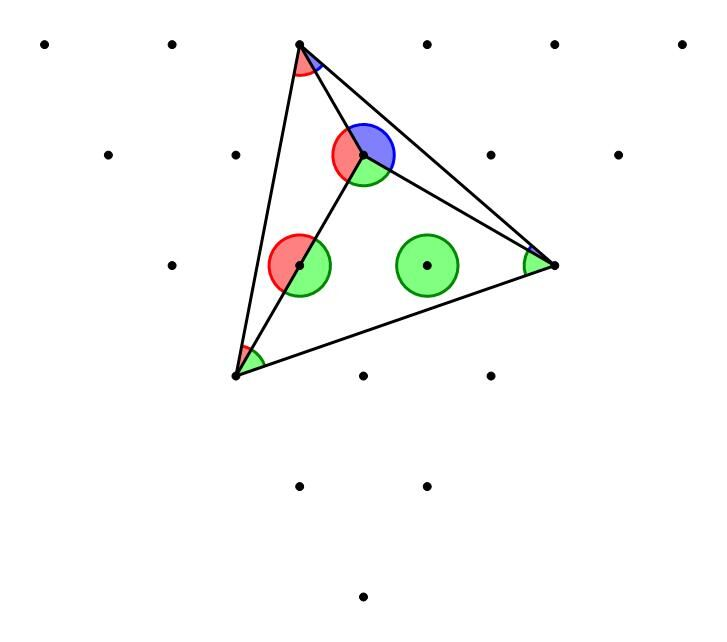
\includegraphics[width=0.4\linewidth]{140}
\end{center}

$ \displaystyle  \sum a^{5}b^{2}-\displaystyle  \sum a^{3}b^{3}c= $
\renewcommand*{\arraystretch}{1.732}\[\left[\begin{matrix}
	\begin{tabular}{ccccccccccccccc}
		0& &0& &1& &0& &0& &0& &0& &0\\
		&0& &0& &0& &-1& &0& &0& &0&\\
		& &0& &0& &0& &0& &0& &1& &\\
		& & &0& &-1& &0& &-1& &0& & &\\
		& & & &0& &0& &0& &0& & & &\\
		& & & & &1& &0& &0& & & & &\\
		& & & & & &0& &0& & & & & &\\
		& & & & & & &0& & & & & & &\\
	\end{tabular}
\end{matrix}\right]\]


于是其实我们已经暗中得到了一个结论:如果三个$ 1 $和三个$ -1 $构成的正三角形共中心,且$ 1 $的套住$ -1 $的,那么这个非负性成立,证明的话直接根据奔驰定理给出三个均值局部即可,米尔黑德定理就和它类似,如果一个轮换对称六边形套住另一个,那么非负性成立,以上说的都是观察手段,当然不要在解答过程里这样推理,上面这种的话写三个均值相加,或者直接$ (\displaystyle \sum a^{2}b^{2}-\displaystyle \sum a^{4}b^{2}c) $

这是米尔黑德的例子:
\begin{center}
	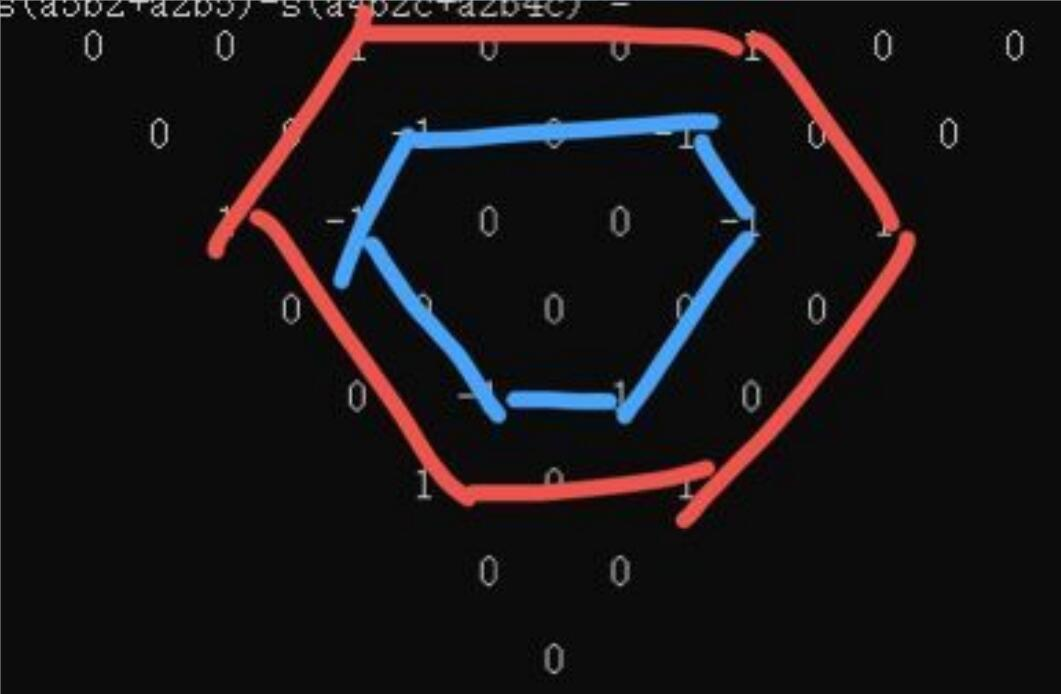
\includegraphics[width=0.45\linewidth]{160}
\end{center}
以上两个结论(正三角形的、“轮换对称六边形”的)事实上暗示了一个道理,靠外的项更贵,靠内的项更贱,就是说在外面的项可以轻易地大过里面的,因此靠外的负项应当小心处理、优先处理,靠外的正项应该尽可能有效利用。\\

\section{$ (a-b)^{2n}$结构}
\subsection{$ (a-b)^{2n}$}
如$ (a-b)^{4} $、$ (a-b)^{6} $这类,在分拆中使用这样的结构可以更有效地利用靠外的正项,比如我们对比一下,如果是用$ (a-b)^{4} $,得到的就是这样
$ (a-b)^{4}= $
\renewcommand*{\arraystretch}{1.732}\[\left[\begin{matrix}
	1& &-4& &6& &-4& &1\\
	&0& &0& &0& &0&\\
	& &0& &0& &0& &\\
	& & &0& &0& & &\\
	& & & &0& & & &\\
\end{matrix}\right]\]
可以理解为拿1个$ a^{4} $、1个$ b^{4} $、6个$ a^{2}b^{2} $解决了4个$ a^{3}b $和4个$ ab^{3} $但如果是用均值做类似的事

$ (a-b)^{2}(a^{2}+b^{2})= $
\renewcommand*{\arraystretch}{1.732}\[\left[\begin{matrix}
	1& &-2& &2& &-2& &1\\
	&0& &0& &0& &0&\\
	& &0& &0& &0& &\\
	& & &0& &0& & &\\
	& & & &0& & & &\\
\end{matrix}\right]\]
就变成拿$ 1 $个$ a^{4} $、$ 1 $个$ b^{4} $、$ 2 $个$ a^{2}b^{2} $解决了$ 2 $个$ a^{3}b $和2个$ ab^{3} $
如果带着靠外项更贵的心态来看,显然上面的性价比更高,况且实际上它们作差就是$ 2ab(a-b)^{2} $,所以显然$ (a-b)^{4} $更紧一些,这里应当感受的是$ n $为不小于$ 2 $的正整数时$ (a-b)^{2n} $比均值紧很多,而且$ n $越大越紧。这只是考虑用$ a^{4} $、$ b^{4} $、$ a^{2}b^{2} $去攻击$ a^{3}b $和$ ab^{3} $
那就近的话自然就是这两组均值\\
\subsection{习题}
*这些习题并不是都能用这节讲到的方法解决,对于搞不定的可以思考能如何投机取巧
$(1) \displaystyle  \sum a^{2} \geq \displaystyle \sum a b \\
(2)  \displaystyle \sum a^{3} \geq \displaystyle \sum a^{2} b \\
(3)  \displaystyle \sum a^{3} b \geq \displaystyle \sum a^{2} b c \\
(4)  \displaystyle \sum a^{5}+2  \displaystyle \sum a^{2} b^{2} c \geq 3  \displaystyle \sum a^{3} b c \\
(5) \displaystyle \sum a^{4}+3 \displaystyle \sum a^{2} b^{2} \geq 2 \displaystyle \sum a b\left(a^{2}+b^{2}\right) \\
(6)  \displaystyle \sum a^{5}+5  \displaystyle \sum a^{3} b^{2} \geq 6  \displaystyle \sum a^{3} b c \\
(7)  \displaystyle \sum a^{5}+3 \displaystyle \sum a^{2} b^{2} c \geq 4  \displaystyle \sum a^{3} b c \\
(8)  \displaystyle \sum a^{5}+8 \displaystyle \sum a^{3} b^{2} \geq 9 \displaystyle \sum a^{3} b c \\
(9)  \displaystyle \frac{\displaystyle \sum a^{2} \displaystyle \sum a^{3}}{3 a b c} \geq 4 \displaystyle \sum a^{2}-3 \displaystyle \sum a b \\
(10)  \displaystyle \sum a^{5}+10  \displaystyle \sum a^{3} b^{2} \geq 11  \displaystyle \sum a^{3} b c \\ $
\\
$(1)\dfrac{1}{2} \displaystyle \sum (a-b)^{2}$\\
(2)aab配\\
$(5)(a-b)^{2}(a-c)^{2}$,同时它也等于$\dfrac{1}{2} \displaystyle \sum (a-b)^{4}$
其实这个更容易想到,因为看系数阵的话只有外边一圈,容易想到是不是能分成三条边处理\\
(6)恰好就是三个均值,这里可以利用面积配系数,很明显张成的三块面积$1:2:3$
   \begin{center}
   	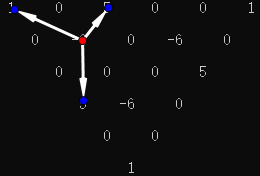
\includegraphics[width=0.5\linewidth]{180}
   \end{center}
(7)可以发现它是(4)的加强,而(4)我们是拆成三个均值完成的,可见相同的方法将失效,把这样几个平方相乘的话强度会增加,可见$\displaystyle \sum a(a-b)^{2}(a-c)^{2}$会是一个比较强的结构,\\
实际上拆下这个$\displaystyle \sum a(a-b)^{2}(a-c)^{2}$之后剩这些:\\
 $\displaystyle \sum (a^{5}+3a^{2}b^{2}c-4a^{3}bc)-\displaystyle \sum (a(a-b)^{2}(a-c)^{2})=$\\
 \renewcommand*{\arraystretch}{1.732}\[\left[\begin{matrix}
 	\begin{tabular}{ccccccccccccc}
 		0& &2& &-1& &-1& &2& &0\\
 		&2& &-8& &6& &-8& &2&\\
 		& &-1& &6& &6& &-1& &\\
 		& & &1& &-8& &-1& & &\\
 		& & & &2& &2& & & &\\
 		& & & & &0& & & & &\\
 	\end{tabular}
 \end{matrix}\right]\]
实际上和$ (a-b)^{2}(a-c)^{2} $的强度差不多,所以如果不是形状特别适合$ (a-b)^{2}(a-c)^{2} $的话一般先从$ (a-b)^{2n} $这个东西试起,如此一来计算量会小一些,说回这个,中间那几个$-8$和$+6$
  \begin{center}
  	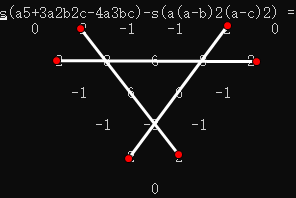
\includegraphics[width=0.4\linewidth]{190}
  \end{center}
正好便于我们拆$\displaystyle \sum c(a-b)^{4}$出来,毕竟$\displaystyle \sum c(a-b)^{4}$正好是$[1,-4,6,-4,1]$,然后就剩:\\
  $ \displaystyle \sum (a^{5}+3a^{2}b^{2}c-4a^{3}bc)-\displaystyle \sum (a(a-b)^{2}(a-c)^{2})-\displaystyle \sum (c(a-b)^{4}) = $
  \renewcommand*{\arraystretch}{1.732}\[\left[\begin{matrix}
  	\begin{tabular}{ccccccccccccc}
  		0& &1& &-1& &-1& &1& &0\\
  		&1& &0& &0& &0& &1&\\
  		& &-1& &0& &0& &-1& &\\
  		& & &-1& &0& &-1& & &\\
  		& & & &1& &1& & & &\\
  		& & & & &0& & & & &\\
  	\end{tabular}
  \end{matrix}\right]\]
$ \displaystyle \sum ab(a-b)(a^{2}-b^{2}) $搞定。虽然之前没强调,不过大家应该知道$ (a^{m}-b^{m})(a^{n}-b^{n}) $非负,形状为对称的“$ 1 $…$ -1 $…$ -1 $…$ 1 $”,\\
那么再说说另一种做法
$ \displaystyle \sum (a^{5}+3a^{2}b^{2}c-4a^{3}bc)= $
  \renewcommand*{\arraystretch}{1.732}\[\left[\begin{matrix}
  	\begin{tabular}{ccccccccccccc}
  		1& &0& &0& &0& &0& &1\\
  		&0& &-4& &3& &-4& &0&\\
  		& &0& &3& &3& &0& &\\
  		& & &0& &-4& &0& & &\\
  		& & & &0& &0& & & &\\
  		& & & & &1& & & & &\\
  	\end{tabular}
  \end{matrix}\right]\]
从一开始就考虑靠$ (a-b)^{4} $来发挥里面的3,当然,因为只有3所以拿半个,也就是$ \dfrac{1}{2} \displaystyle \sum c(a-b)^{4} $,于是中间全没了,剩这个:
 \renewcommand*{\arraystretch}{1.732}\[\left[\begin{matrix}
	\begin{tabular}{ccccccccccccc}
		1& &$ -\dfrac{1}{2} $& &0& &0& &$ -\dfrac{1}{2} $& &1\\
		&$ -\dfrac{1}{2} $& &0& &0& &0& &$ -\dfrac{1}{2} $&\\
		& &0& &0& &0& &0& &\\
		& & &0& &0& &0& & &\\
		& & & &$ -\dfrac{1}{2} $& &$ -\dfrac{1}{2} $& & & &\\
		& & & & &1& & & & &\\
	\end{tabular}
  \end{matrix}\right]\]
也就是$ \displaystyle \dfrac{1}{2} \displaystyle \sum (a-b)(a^{4}-b^{4}) $也结束了\\
(8)是(6)的加强,我们可以考虑用$ (a-b)^{4} $来消耗最外面的$ a^5 $,那比方说我们尝试$ \displaystyle \sum a(a-b)^{4} $会导致变成这样:\\
$  \displaystyle \sum (a^{5}+8 a^{3} b^{2}-9a^{3}bc)-\displaystyle \sum a(a-b)^{4}=$
  \renewcommand*{\arraystretch}{1.732}\[\left[\begin{matrix}
  	\begin{tabular}{ccccccccccccc}
  		0& &4& &2& &4& &-1& &0\\
  		&-1& &-9& &0& &-9& &4&\\
  		& &4& &0& &0& &2& &\\
  		& & &2& &-9& &4& & &\\
  		& & & &4& &-1& & & &\\
  		& & & & &0& & & & &\\
  	\end{tabular}
  \end{matrix}\right]\]
这个$ -1 $脱离了正项的凸包,意味着放过头了,这肯定不行了,因此吸取教训(只是演示一下可能的错误)。拆$ \dfrac{1}{2}\displaystyle \sum (a+b)(a-b)^{4} $,这样的话一方面不会出现上面这样的翻车。
  \begin{center}
  	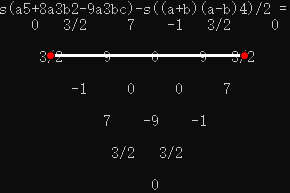
\includegraphics[width=0.4\linewidth]{200}
  \end{center}
另一方面$ a^{4}b $和$ ab^{4} $上系数相等了,便于我们再去拿$ c(a-b)^{4} $,后面计算不说了,顺便我们知道 \\
$ \dfrac{1}{5} \displaystyle \sum (4a+b)(a-b)^{4} $是整系数的\\
$ \dfrac{1}{5} \displaystyle \sum (3a+2b)(a-b)^{4} $\\
$ \dfrac{1}{5} \displaystyle \sum (2a+3b)(a-b)^{4} $\\
$ \dfrac{1}{5} \displaystyle \sum (a+4b)(a-b)^{4} $\\
甚至这几个都是整系数的。
以至于可以搞出$  \displaystyle \sum (a^{5}+8 a^{3} b^{2}-9a^{3}bc)- \displaystyle \sum \dfrac{1}{5}(3a+2b+5c)(a-b)^{4}= $
  \renewcommand*{\arraystretch}{1.732}\[\left[\begin{matrix}
  	\begin{tabular}{ccccccccccccc}
  		0& &1& &6& &0& &0& &0\\
  		&0& &-1& &-6& &-1& &1&\\
  		& &0& &-6& &-6& &6& &\\
  		& & &6& &-1& &0& & &\\
  		& & & &1& &0& & & &\\
  		& & & & &0& & & & &\\
  	\end{tabular}
  \end{matrix}\right]\]
\section{舒尔不等式}
\subsection{简单的舒尔不等式}
我们探索到这个阶段,很容易想到一个简单的问题,齐三次的,轮换对称的问题有没有通用的配方办法。考虑到必须有$ F(a,b,0) \geq 0 $,我们容易发现“最强”的问题就是
\renewcommand*{\arraystretch}{1.732}\[\left[\begin{matrix}
	1& &-1& &-1& &1\\
	&-1& &3& &-1&\\
	& &-1& &-1& & \\
	& & &1& & &\\
\end{matrix}\right]\]
这时候我们便要聚焦这个问题,容易发现它是没法靠均值解决的(不升次数的话)。\\
看过预备知识我们发现这个东西叫做舒尔不等式,考虑到它在系数阵里的形状相当有特点,我们便将其引入配方技术之中,毕竟它便于使用,承认这是配方法的一部分就省去了将它特地配方的多余操作。\\
schur在系数阵视角下形状独特,
比如三次的像这样
$ \displaystyle \sum (a(a-b)(a-c))= $
\renewcommand*{\arraystretch}{1.732}\[\left[\begin{matrix}
	1& &-1& &-1& &1\\
	&-1& &3& &-1&\\
	& &-1& &-1& & \\
	& & &1& & &\\
\end{matrix}\right]\]
四次的像这样
$ \displaystyle \sum (a^{2}(a-b)(a-c))= $
\renewcommand*{\arraystretch}{1.732}\[\left[\begin{matrix}
	1& &-1& &0& &-1& &1\\
	&-1& &1& &1& &-1&\\
	& &0& &1& &0& &\\
	& & &-1& &-1& & &\\
	& & & &1& & & &\\
\end{matrix}\right]\]
五次的像这样
$ \displaystyle \sum (a^{3}(a-b)(a-c))= $
\renewcommand*{\arraystretch}{1.732}\[\left[\begin{matrix}
	\begin{tabular}{ccccccccccccc}
		1& &-1& &0& &0& &-1& &1\\
		&-1& &1& &0& &1& &-1&\\
		& &0& &0& &0& &0& &\\
		& & &0& &1& &0& & &\\
		& & & &-1& &-1& & & &\\
		& & & & &1& & & & &\\
	\end{tabular}
\end{matrix}\right]\]
这里再顺便偏个题,schur的一个有趣配方,如果将三次的schur乘上$ (a+b)(a+c)(b+c) $你会惊讶地发现,乘出来的非零项比schur本身还少
\renewcommand*{\arraystretch}{1.732}\[\left[\begin{matrix}
	\begin{tabular}{ccccccccccccc}
		0& &1& &0& &-2& &0& &1& &0\\
		&1& &0& &0& &0& &0& &1&\\
		& &0& &0& &0& &0& &0& &\\
		& & &-2& &0& &0& &-2& & &\\
		& & & &0& &0& &0& & & &\\
		& & & & &1& &1& & & & &\\
		& & & & & &0& & & & & &\\
	\end{tabular}
\end{matrix}\right]\]
结果是这个,不过这个就不要追问为什么了,偶然发现的,高次舒尔就没找到类似的恒等式了。
\subsection{一道题}
证明下式$ \geq 0 $\\
\renewcommand*{\arraystretch}{1.732}\[\left[\begin{matrix}
	\begin{tabular}{ccccccccccccc}
		0&  &1  &  & 0 &  & -2 &  & 0 &  & 1 &  & 0\\
		&1  &  & -2 &  & 1 &  & 1 &  & -2 &  & 1 & \\
		&  & 0 &  & 1 &  &  0&  &  1&  &  0&  & \\
		&  &  &  -2 &  & 1 &  & 1 &  & -2  &  &  & \\
		&  &  &  &  0&  &-2  &  & 0 &  &  &  & \\
		&  &  &  &  &  1&  &1  &  &  &  &  & \\
		&  &  &  &  &  &  0&  &  &  &  &  & \\
	\end{tabular}
\end{matrix}\right]\]

拿一个$ (a-b)^{2}(a-c)^{2}(b-c)^{2} $出来,
提完会是这样,
\renewcommand*{\arraystretch}{1.732}\[\left[\begin{matrix}
	\begin{tabular}{ccccccccccccc}
		0&  &1  &  & -1 &  & 0 &  & -1 &  & 1 &  & 0\\
		&1  &  & 0 &  & -1 &  & -1 &  & 0 &  & 1 & \\
		&  & -1 &  & -1 &  &  6&  &  -1&  &  -1&  & \\
		&  &  &  0 &  & -1 &  & -1 &  & 0  &  &  & \\
		&  &  &  &  -1&  &0  &  & -1 &  &  &  & \\
		&  &  &  &  &  1&  &1  &  &  &  &  & \\
		&  &  &  &  &  &  0&  &  &  &  &  & \\
	\end{tabular}
\end{matrix}\right]\]
那么$ ab $边上的$ 1,-1,0,-1,1 $暗示了schur:
$$ (x-y)^{2}(x-z)^{2}(y-z)^{2}+\displaystyle \sum x y \cdot \displaystyle \sum x^{2}(x-y)(x-z)+x y z \cdot \displaystyle \sum x(x-y)(x-z) \geq 0 $$
重点是那三个菱形,其它的是0
\begin{center}
	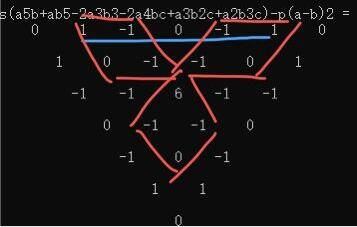
\includegraphics[width=0.5\linewidth]{170}
\end{center}

于是这里就会考虑这个了,这是$ab$Schur$4 $,那么对称的也扣掉,就是$ \displaystyle \sum ab·$ schur $4 $,这样一来最外面一圈就都没了,实际上里面刚好剩下一个三次的schur,那就好了,也就是这样
$ (x-y)^{2}(x-z)^{2}(y-z)^{2}+\displaystyle \sum x y \cdot \displaystyle \sum x^{2}(x-y)(x-z)+x y z \cdot \displaystyle \sum x(x-y)(x-z) \geq 0 $
\\
\subsection{习题}
\noindent (1) $2 \displaystyle  \sum a^{3}+3 a b c \geq 3\displaystyle  \sum  a^{2} b$\\
(2) $2\displaystyle  \sum  a^{4}+\displaystyle  \sum  a^{2} b c \geq 3 \sum a^{2} b^{2}$\\
(3) $ \displaystyle  \sum \dfrac{1}{(a+b)^{2}} \geq \dfrac{9}{4 \displaystyle  \sum a b}$\\
(4) $\displaystyle  \sum  a^{6}+3 a^{2} b^{2} c^{2} \geq 2 \displaystyle  \sum  a^{3} b^{3}$\\
(5) $\displaystyle  \sum a^{5}+\displaystyle  \sum  a^{2} b^{2} c \geq \displaystyle  \sum a^{2} b^{2}(a+b)$\\
(6) $ \displaystyle  \sum  \dfrac{a^{2} b^{2}}{c}+\displaystyle  \sum  a^{3}+6 a b c \geq 2 \displaystyle  \sum  a b(a+b)$\\
(7) $4 \displaystyle  \sum a^{5}+2\sum a^{2} b^{2} c \geq 3 \displaystyle  \sum  a b\left(a^{3}+b^{3}\right)$\\
(8) $\displaystyle  \sum  a^{5}+2  \displaystyle  \sum  a^{2} b^{2} c \geq \displaystyle  \sum  a^{3}\left(b^{2}+b c+c^{2}\right)$\\
(9) $\displaystyle  \sum a^{5}+6  \displaystyle  \sum a^{2} b^{2} c \geq 7 \displaystyle  \sum  a^{3} b c$\\
(10) $21 a b c+\dfrac{a^{5}}{b c} \geq 4\displaystyle  \sum  a b(a+b)$\\
\noindent (1)  \renewcommand*{\arraystretch}{1.732}\[\left[\begin{matrix}
	2& &-3& &0& &2\\
	&0& &3& &-3&\\
	& &-3& &0& & \\
	& & &2& & &\\
\end{matrix}\right]\] 
上次也说明了,仅仅用简单均值不可能利用上中间的3,所以提出一个schur,变成三个$ [1,-2,1] $
 \renewcommand*{\arraystretch}{1.732}\[\left[\begin{matrix}
	1& &-2& &1& &1\\
	&1& &0& &-2&\\
	& &-2& &1& & \\
	& & &1& & &\\
\end{matrix}\right]\]
即$ \displaystyle \sum a(a-b)(a-c)+\displaystyle \sum a^{2}(a-b)\geq 0 $\\
(2)\renewcommand*{\arraystretch}{1.732}\[\left[\begin{matrix}
	2& &0& &-3& &0& &2\\
	&0& &1& &1& &0&\\
	& &-3& &1& &-3& &\\
	& & &0& &0& & &\\
	& & & &2& & & &\\
\end{matrix}\right]\]
一样的道理,要把中间三个1用上,所以拿一份schur,然后也是只需均值\\
$ \displaystyle  \sum (2a^{4}+a^{2}bc-3a^{2}b^{2})-\displaystyle  \sum a^{2}(a-b)(b-c) $
\renewcommand*{\arraystretch}{1.732}\[\left[\begin{matrix}
	1& &1& &-3& &1& &1\\
	&1& &0& &0& &1&\\
	& &-3& &0& &-3& &\\
	& & &1& &1& & &\\
	& & & &1& & & &\\
\end{matrix}\right]\]
即$ \displaystyle \sum a^{2}(a-b)(a-c)+\displaystyle \sum a^{4}+\displaystyle \sum (a^{3}b+ab^{3})\geq \displaystyle \sum a^{2}(a-b)(a-c)+3\displaystyle \sum a^{2}b^{2}$\\
(3)是iran96,化整后变成这样一个六次的问题\\
$ 4\displaystyle \sum ab\displaystyle \sum (a+b)^{2}(a+c)^{2}-9\prod (a+b)^{2}= $
\renewcommand*{\arraystretch}{1.732}\[\left[\begin{matrix}
	\begin{tabular}{ccccccccccccc}
		0& &4& &-1& &-6& &-1& &4& &0\\
		&4& &2& &-2& &-2& &2& &4&\\
		& &-1& &-2& &6& &-2& &-1& &\\
		& & &-6& &-2& &-2& &-6& & &\\
		& & & &-1& &2& &-1& & & &\\
		& & & & &4& &4& & & & &\\
		& & & & & &0& & & & & &\\
	\end{tabular}
\end{matrix}\right]\]
首先我们观察到第一行总和为$ 0 $,即$ F(1,1,0)=0 $,即$ a=b $且$ c=0 $时取等
\begin{center}
	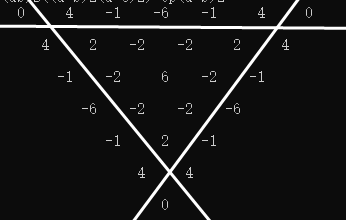
\includegraphics[width=0.4\linewidth]{220}
\end{center}
然后再一看,中间就是一个schur的两倍,故这样分成四块分别解决即可\\
(4)\renewcommand*{\arraystretch}{1.732}\[\left[\begin{matrix}
	\begin{tabular}{ccccccccccccc}
		1& &0& &0& &-2& &0& &0& &1\\
		&0& &0& &0& &0& &0& &0&\\
		& &0& &0& &3& &0& &0& &\\
		& & &-2& &0& &0& &-2& & &\\
		& & & &0& &0& &0& & & &\\
		& & & & &0& &0& & & & &\\
		& & & & & &1& & & & & &\\
	\end{tabular}
\end{matrix}\right]\]
\begin{center}
	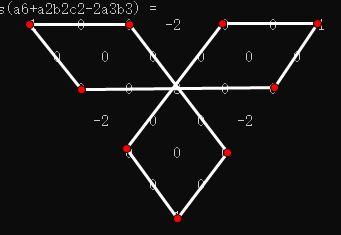
\includegraphics[width=0.5\linewidth]{230}
\end{center}
\begin{center}
	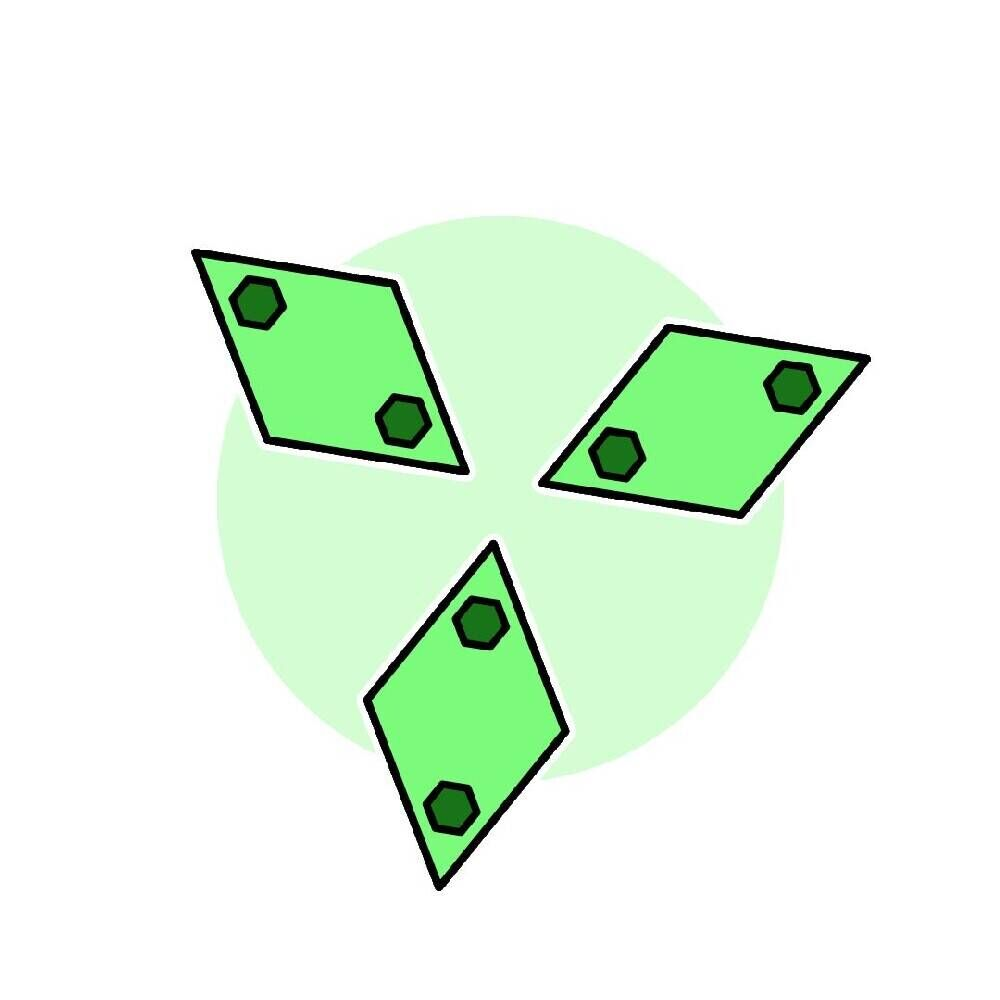
\includegraphics[width=0.4\linewidth]{210}
\end{center}
还是一样的道理,关键在于如何利用中间的3,那么自然地想到这样的schur,也就是减掉$ \displaystyle  \sum a^{2}(a^{2}-b^{2})(a^{2}-c^{2}) $
\renewcommand*{\arraystretch}{1.732}\[\left[\begin{matrix}
	\begin{tabular}{ccccccccccccc}
		0& &0& &1& &-2& &1& &0& &0\\
		&0& &0& &0& &0& &0& &0&\\
		& &1& &0& &0& &0& &1& &\\
		& & &-2& &0& &0& &-2& & &\\
		& & & &1& &0& &1& & & &\\
		& & & & &0& &0& & & & &\\
		& & & & & &0& & & & & &\\
	\end{tabular}
\end{matrix}\right]\]
取出之后剩下三个$ [1,-2,1] $结束\\
即$\displaystyle  \sum  a^{6}+3 a^{2} b^{2} c^{2} \geq \displaystyle  \sum (a^{4}b^{2}+a^{2}b^{4}) \geq 2 \displaystyle  \sum  a^{3} b^{3}$\\
(5)\begin{center}
	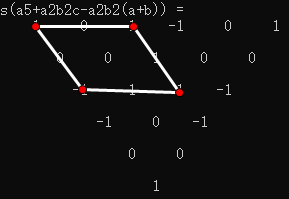
\includegraphics[width=0.5\linewidth]{240}
\end{center}
这是一个舒尔$ \displaystyle  \sum a(a^{2}-b^{2})(a^{2}-c^{2}) $,一共有三个。可以看出即使是像这样的变形,schur在系数阵里依然保持原本的形状规律,这里$ a,b,c $取作$ a^{2},b^{2},c^{2} $,$ t $取$ \dfrac{1}{2} $\\
即$\displaystyle  \sum a^{5}+\displaystyle  \sum  a^{2} b^{2} c -\displaystyle  \sum a^{2} b^{2}(a+b)=\displaystyle  \sum x^{3}(x-y)(x-z)+\displaystyle  \sum x^{2}(y+z)(x-y)(x-z)+\displaystyle  \sum xyz(x-y)(x-z)$\\
(6)\renewcommand*{\arraystretch}{1.732}\[\left[\begin{matrix}
	\begin{tabular}{ccccccccccccc}
		0& &0& &0& &1& &0& &0& &0\\
		&0& &1& &-2& &-2& &1& &0&\\
		& &0& &-2& &6& &-2& &0& &\\
		& & &1& &-2& &-2& &1& & &\\
		& & & &0& &1& &0& & & &\\
		& & & & &0& &0& & & & &\\
		& & & & & &0& & & & & &\\
	\end{tabular}
\end{matrix}\right]\]
这就是两个schur重叠,倒的那个是$ \displaystyle  \sum b^{2}c^{2}(a-b)(a-c) $\\
可以理解为schur定理t=-2\\
$\displaystyle  \sum  b^{2} c^{2}(a-b)(a-c)=a^{2} b^{2} c^{2} \displaystyle  \sum  a^{-2}(a-b)(a-c) $\\
理解为换元也是可以的
$\displaystyle  \sum b^{2} c^{2}(a-b)(a-c)=\displaystyle  \sum b c(b c-a b)(b c-a c)$\\
(7)\renewcommand*{\arraystretch}{1.732}\[\left[\begin{matrix}
	\begin{tabular}{ccccccccccccc}
		4& &-3& &0& &0& &-3& &4\\
		&-3& &0& &2& &0& &-3&\\
		& &0& &2& &2& &0& &\\
		& & &0& &0& &0& & &\\
		& & & &-3& &-3& & & &\\
		& & & & &4& & & & &\\
	\end{tabular}
\end{matrix}\right]\]
提一个4倍schur:$ \displaystyle \sum (4a^{5}+2a^{2}b^{2}c-3ab(a^{3}+b^{3}))-4\displaystyle \sum (a^{3}(a-b)(a-c))= $
\renewcommand*{\arraystretch}{1.732}\[\left[\begin{matrix}
	\begin{tabular}{ccccccccccccc}
		0& &1& &0& &0& &1& &0\\
		&1& &-4& &2& &-4& &1&\\
		& &0& &2& &2& &0& &\\
		& & &0& &-4& &0& & &\\
		& & & &1& &1& & & &\\
		& & & & &0& & & & &\\
	\end{tabular}
\end{matrix}\right]\]
很明显$ 4 $个$ 1 $攻击一个$ -4 $,六个均值,也可以说是三个四元均值\\
那么如果换个思路,为了把$ -3 $弄掉而提$ 3 $倍schur:\\
$ \displaystyle \sum (4a^{5}+2a^{2}b^{2}c-3ab(a^{3}+b^{3}))-3\displaystyle \sum (a^{3}(a-b)(a-c))= $
\renewcommand*{\arraystretch}{1.732}\[\left[\begin{matrix}
	\begin{tabular}{ccccccccccccc}
		1& &0& &0& &0& &0& &1\\
		&0& &-3& &2& &-3& &0&\\
		& &0& &2& &2& &0& &\\
		& & &0& &-3& &0& & &\\
		& & & &0& &0& & & &\\
		& & & & &1& & & & &\\
	\end{tabular}
\end{matrix}\right]\]
剩下就是这样,正好也是均值,重心,三元均值。\\
甚至我们可以提2倍schur,为了用到中间的2,取第五题那样的schur:\\
$ \displaystyle \sum (4a^{5}+2a^{2}b^{2}c-3ab(a^{3}+b^{3}))-
 2\displaystyle \sum a(a^{2}-b^{2})(a^{2}-c^{2})=$
 \renewcommand*{\arraystretch}{1.732}\[\left[\begin{matrix}
 	\begin{tabular}{ccccccccccccc}
 		2& &-3& &2& &2& &-3& &2\\
 		&-3& &0& &0& &0& &2&\\
 		& &2& &0& &0& &-3& &\\
 		& & &2& &0& &2& & &\\
 		& & & &-3& &-3& & & &\\
 		& & & & &2& & & & &\\
 	\end{tabular}
 \end{matrix}\right]\]
然后可以拆成三条$ [1,-3,2,2,-3,1] $,这恰好是$ (a+b)(a-b)^{4}$\\
注:提出的结构必须契合不等式的取等,首先注意到$ ab $边上和为$ 0 $,因此你要动角上那个1的话,不可能用均值或者$ (a-b)^{2n} $,因为它是二元对称的,所以总之先考虑$ (a+b)(a-b)^{4}$这个通常来说最强的东西\\
(8)\renewcommand*{\arraystretch}{1.732}\[\left[\begin{matrix}
	\begin{tabular}{ccccccccccccc}
		1& &0& &-1& &-1& &0& &1\\
		&0& &-1& &2& &-1& &0&\\
		& &-1& &2& &2& &-1& &\\
		& & &-1& &0& &-1& & &\\
		& & & &0& &0& & & &\\
		& & & & &1& & & & &\\
	\end{tabular}
\end{matrix}\right]\]
显然不能提出三个大schur:$ \displaystyle \sum a(a^{2}-b^{2})(a^{2}-c^{2}) $,提完会当场去世。\\
可以试试提$ \displaystyle \sum a^{3}(a-b)(a-c) $:
\renewcommand*{\arraystretch}{1.732}\[\left[\begin{matrix}
	\begin{tabular}{ccccccccccccc}
		0& &1& &-1& &-1& &1& &0\\
		&1& &-2& &2& &-2& &1&\\
		& &-1& &2& &2& &-1& &\\
		& & &-1& &-2& &-1& & &\\
		& & & &1& &1& & & &\\
		& & & & &0& & & & &\\
	\end{tabular}
\end{matrix}\right]\]
看到这个我们顶多想到拆三个小schur,但也会去世。(实际上可以配方,但现在先假装不会)于是我们还有最后一个选择\\
拆三个四阶的schur:
$ \displaystyle \sum  (a^{5}+2a^{2}b^{2}c-a^{3}(b^{2}+bc+c^{2}))-\displaystyle \sum a \displaystyle \sum  a^{2}(a-b)(a-c)=0 $
然后拆完发现啥都没了,拆了三个这样的四阶schur:
\begin{center}
	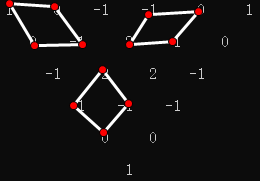
\includegraphics[width=0.4\linewidth]{250}
\end{center}
反正也就这么一个选择,所以有因式$ \displaystyle \sum a $,这提示我们做题时要先因式分解\\
(9)\renewcommand*{\arraystretch}{1.732}\[\left[\begin{matrix}
	\begin{tabular}{ccccccccccccc}
		1& &0& &0& &0& &0& &1\\
		&0& &-7& &6& &-7& &0&\\
		& &0& &6& &6& &0& &\\
		& & &0& &-7& &0& & &\\
		& & & &0& &0& & & &\\
		& & & & &1& & & & &\\
	\end{tabular}
\end{matrix}\right]\]
这是上次均值习题的升级版,提一个schur:
$ \displaystyle \sum (a^{5}+6a^{2}b^{2}c+7a^{3}bc)-\displaystyle \sum a^{3}(a-b)(a-c)= $
\renewcommand*{\arraystretch}{1.732}\[\left[\begin{matrix}
	\begin{tabular}{ccccccccccccc}
		0& &1& &0& &0& &1& &0\\
		&1& &-8& &6& &-8& &1&\\
		& &0& &6& &6& &0& &\\
		& & &0& &-8& &0& & &\\
		& & & &1& &1& & & &\\
		& & & & &0& & & & &\\
	\end{tabular}
\end{matrix}\right]\]
然后是三个[1,-4,6,-4,1]\\
(10)齐次化即$ \displaystyle \sum a^{6}+21a^{2}b^{2}c^{2}-4\displaystyle \sum a^{2}b^{2}(ac+bc)= $
\renewcommand*{\arraystretch}{1.732}\[\left[\begin{matrix}
	\begin{tabular}{ccccccccccccc}
		1& &0& &0& &0& &0& &0& &1\\
		&0& &0& &-4& &-4& &0& &0&\\
		& &0& &-4& &21& &-4& &0& &\\
		& & &0& &-4& &-4& &0& & &\\
		& & & &0& &0& &0& & & &\\
		& & & & &0& &0& & & & &\\
		& & & & & &1& & & & & &\\
	\end{tabular}
\end{matrix}\right]\]
和上一题差不多,一个schur和三个$ [1,-4,6,-4,1] $
\section{配方}
\subsection{平方}
下面是$ (a-b)^{2} $、$ (a+b-2c)^{2} $、$ (a+2b-3c)^{2} $括号内的系数阵,
\renewcommand*{\arraystretch}{1.732}\[\left[\begin{matrix}
	1& &-2& &1\\
	&0& &0&\\
	& &0& &\\
\end{matrix}\right]\]
\renewcommand*{\arraystretch}{1.732}\[\left[\begin{matrix}
	1& &2& &1\\
	&-4& &-4&\\
	& &4& &\\
\end{matrix}\right]\]
\renewcommand*{\arraystretch}{1.732}\[\left[\begin{matrix}
	1& &4& &4\\
	&-6& &-12&\\
	& &9& &\\
\end{matrix}\right]\]
试观察其特点
\begin{center}
	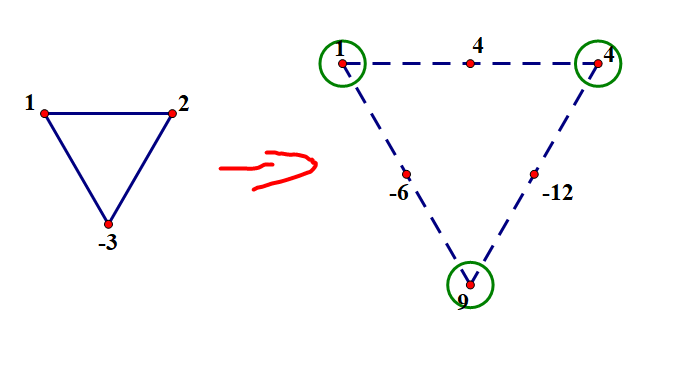
\includegraphics[width=0.5\linewidth]{260}
\end{center}
首先把要平方的阵放大一倍,在对应位置(在大阵上可以称作“桩”)写上小阵各项的平方,然后在每对桩的中点处加上小阵对应数的乘积的两倍,通过完全平方公式不难理解这个规律。值得注意的是,位于凸包顶点处的数必定满足大阵系数为小阵系数的平方。\\
再比如\\
\begin{center}
	$ \left[\begin{matrix}
	1& &2& &0\\
	&0& &-3&\\
	& &0& &\\
\end{matrix}\right]^{2} =
\left[\begin{matrix}
1& &4& &4& &0& &0\\
&0& &-6& &-12& &0&\\
& &0& &0& &9& &\\
& & &0& &0& & &\\
& & & &0& & & &\\
\end{matrix}\right]$
\end{center}
\begin{center}
	$ \left[\begin{matrix}
		1& &0& &-1\\
		&-1& &1&\\
		& &0& &\\
	\end{matrix}\right]^{2} =
	\left[\begin{matrix}
		1& &0& &-2& &0& &1\\
		&-2& &2& &2& &-2&\\
		& &1& &-2& &1& &\\
		& & &0& &0& & &\\
		& & & &0& & & &\\
	\end{matrix}\right]$
\end{center}
再来个有中点重合的$ (a^{2}-ab-ac+bc)^{2} $(算的时候可以装作不知道它可以分解)
\begin{center}
	$ \left[\begin{matrix}
		1& &-1& &0\\
		&-1& &1&\\
		& &0& &\\
	\end{matrix}\right]^{2} =
	\left[\begin{matrix}
		1& &-2& &1& &0& &0\\
		&-2& &4& &-2& &0&\\
		& &1& &-2& &1& &\\
		& & &0& &0& & &\\
		& & & &0& & & &\\
	\end{matrix}\right]$
\end{center}
再如$ (2a^{2}-3ab-4ac+5bc)^{2} $
\begin{center}
	$ \left[\begin{matrix}
	2& &-3& &0\\
	&-4& &5&\\
	& &0& &\\
\end{matrix}\right]^{2}=
\left[\begin{matrix}
4& &-12& &9& &0& &0\\
&-16& &44& &-30& &0&\\
& &16& &-40& &25& &\\
& & &0& &0& & &\\
& & & &0& & & &\\
\end{matrix}\right] $
\end{center}
以及$ (2a^{2}-2ac
+3bc+ab+2b^{2})^{2} $
\begin{center}
	$ \left[\begin{matrix}
		2& &1& &2\\
		&-2& &3&\\
		& &0& &\\
	\end{matrix}\right]^{2}=
	\left[\begin{matrix}
		4& &4& &9& &4& &4\\
		&-8& &8& &-2& &12&\\
		& &4& &-12& &9& &\\
		& & &0& &0& & &\\
		& & & &0& & & &\\
	\end{matrix}\right] $
\end{center}
希望能感受到这种方法相对于写代数式的便利,而且这样写也便于后续操作,例如求轮换和之类
\subsection{配方法引入}
那么开始配方法的引入,这要从“想出一个$ (a,b,c)=(1,2,0) $能取等的不等式”开始,想要的还是三元齐次轮换的,那么自然就希望$ F(a,b,0) $和$ (2a-b)^{2} $有点关系。但角上的数得想等,不可能一个1一个4,最终自然就造出了这个:
\renewcommand*{\arraystretch}{1.732}\[
\left[\begin{matrix}
	0& &4& &-4& &1& &0\\
	&1& &-1& &-1& &4&\\
	& &-4& &-1& &-4& &\\
	& & &4& &1& & &\\
	& & & &0& & & &\\
\end{matrix}\right]
\]
写出来的时候尚且没有确定它是否是非负的。在在没有引入配方法的时候,均值和舒尔自然是难以解决这个问题的,毕竟它应当有111,210,102,021四个取等。
\\
那么我们回到代数式来看这个问题是啥,把这些$ [4,-4,1] $理在一起,发现它就是$ \displaystyle \sum ab(2a-b)^{2}\geq abc(a+b+c) $,不禁让人想除掉$ abc $,就是$ \displaystyle \sum \dfrac{(2a-b)^{2}}{c} \geq a+b+c $,到这里我们意识到$ \dfrac{(2a-b)^{2}}{c}+c\geq 2(2a-b) $轮换和一下就行了。现在我们反过来看看$ \dfrac{(2a-b)^{2}}{c}c+c\geq 2(2a-b) $对于系数阵而言有何意味,我们知道基本不等式的一个本质是$ a^{2}+b^{2}\geq 2ab $等价于$ (a-b)^{2}\geq 0 $,所以$ \dfrac{(2a-b)^{2}}{c}+c\geq 2(2a-b) $其实就是$\dfrac{(2a-b-c)^{2}}{c}\geq 0 $,把那个$ abc $乘回来,发现我们做的事就是利用了$ \displaystyle \sum ab(2a-b-c)^{2}\geq 0 $,这时候我们再看看它在系数阵里面对应了什么平方的轮换和:
\renewcommand*{\arraystretch}{1.732}\[
\left[\begin{matrix}
	0& &4& &-4& &1& &0\\
	&0& &-4& &2& &0&\\
	& &0& &1& &0& &\\
	& & &0& &0& & &\\
	& & & &0& & & &\\
\end{matrix}\right]
\]
是这个东西的轮换和,这个平方轮换和一下一定是总和为$ 0 $的,而且边上还一定就是这个$ [4,-4,1] $。于是我们知道了如何以系数阵的视角看这个做法,此后我们就可以直接从系数阵上寻求类似的操作了。\\
例如,\\
$ \left[\begin{matrix}
	0& &9& &-6& &1& &0\\
	&1& &-4& &-4& &9&\\
	& &-6& &-4& &-6& &\\
	& & &9& &1& & &\\
	& & & &0& & & &\\
\end{matrix}\right]
=\displaystyle \sum 
\left[\begin{matrix}
	0& &9& &-6& &1& &0\\
	&0& &-12& &4& &0&\\
	& &0& &4& &0& &\\
	& & &0& &0& & &\\
	& & & &0& & & &\\
\end{matrix}\right] $\\
再看这个,
\renewcommand*{\arraystretch}{1.732}\[
\left[\begin{matrix}
	0& &1& &3& &4& &0\\
	&4& &-2& &-2& &1&\\
	& &3& &-2& &3& &\\
	& & &1& &4& & &\\
	& & & &0& & & &\\
\end{matrix}\right]
\]
[1,-3,4]不是完全平方,实际上这个东西是松了,但我们依然可以照[1,-4,4]的那个来配,力求把角上的1和4妥善使用掉,我们拿去三个平方还剩下这个
\renewcommand*{\arraystretch}{1.732}\[
\left[\begin{matrix}
	0& &0& &1& &0& &0\\
	&0& &-1& &-1& &0&\\
	& &1& &-1& &1& &\\
	& & &0& &0& & &\\
	& & & &0& & & &\\
\end{matrix}\right]
\]
自然可以基本不等式搞掉(皮一下的话你可以说它是舒尔),那么再来一个稍微难一点的
\renewcommand*{\arraystretch}{1.732}\[
\left[\begin{matrix}
	0& &13& &-33& &21& &0\\
	&21& &0& &0& &13&\\
	& &-33& &0& &-33& &\\
	& & &13& &21& & &\\
	& & & &0& & & &\\
\end{matrix}\right]
\]
注:$ 4\times 13\times 21-33^{2}=3 $也即$ 4\times 13\times 21>33^{2} $\\
配方,即$ \displaystyle \sum ab(\sqrt{13}a-\sqrt{21}b+(\sqrt{21}-\sqrt{13})c)^{2}+(\sqrt{13\times 21}-\dfrac{33}{2})\displaystyle \sum c^{2}(a-b)^{2} \geq 0$
我们在配方时往往同时带着“把角上正项消去”和“不放过头”两个意图来拆取平方,这点对于配方法非常重要,如\\
\renewcommand*{\arraystretch}{1.732}\[
\left[\begin{matrix}
	0& &10& &-26& &17& &0\\
	&17& &-1& &-1& &10&\\
	& &-26& &-1& &-26& &\\
	& & &10& &17& & &\\
	& & & &0& & & &\\
\end{matrix}\right]
\]
可以先减掉
$\displaystyle \sum 
\left[\begin{matrix}
	0& &9& &-24& &16& &0\\
	&0& &6& &-8& &0&\\
	& &0& &1& &0& &\\
	& & &0& &0& & &\\
	& & & &0& & & &\\
\end{matrix}\right]
=\displaystyle \sum ab
\left[\begin{matrix}
	3& &-4 \\
	& 1&\\
\end{matrix}\right]^{2} $
,然后还是均值\\
那么我们可以总结一下这种角上为0且齐四次轮换的不等式的通法
\begin{center}
	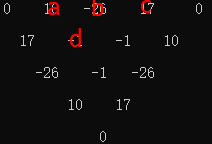
\includegraphics[width=0.3\linewidth]{270}
\end{center}
设这四个位置上的数为$ a,b,c,d $,其中$ a,c> 0 $。首先,考虑到它得以成立,必然要有$ 4ac≥b^{2} $,$ a+b+c+d\geq 0 $。相对地,一旦保证了这四点,就可以拆下一个\\
$ \displaystyle \sum xy(\sqrt{a}x-\sqrt{c}y-(\sqrt{a}-\sqrt{c})z)^{2} $,然后均值即可,此即这类不等式的通法。
那么下面难度升级一下,角上不为零的齐四次轮换对称
\renewcommand*{\arraystretch}{1.732}\[
\left[\begin{matrix}
	1& &-2& &3& &-2& &1\\
	&-2& &0& &0& &-2&\\
	& &3& &0& &3& &\\
	& & &-2& &-2& & &\\
	& & & &1& & & &\\
\end{matrix}\right]
\]
这是$ \dfrac{1}{2}(a-b)^{4} $,但也可以直接考虑$ (\displaystyle \sum (a^{2}-ab))^{2} $
\section{二次元}
\subsection{针对取等的定向配方}
在遇到一些可能不太妙的题目时,除了检查$ f(1,1,1) $这个最平凡的点之外也要注意$ f(a,b,0) $和$ f(a,b,b) $两个特殊的降维情况
看$ f(a,b,b) $时,可以一行一行看总和,然后从下往上念,比如$ [1, -6, 13, -12, 4] $,也就是$ a^{4}-6a^{3}b+13a^{2}b^{2}-12ab^{3}+4b^{4} $,而原不等式有$ a=b=c $取等的话$ f(a,b,b) $必有$ (a-b)^{2} $因式,那么不难发现它其实是$ (a-b)^{2}(a-2b)^{2} $,由此我们会发现原不等式有取等$ (2,1,1) $,
接下来给一个经典的例子
\renewcommand*{\arraystretch}{1.732}\[
\left[\begin{matrix}
	1& &-3& &8& &-3& &1\\
	&-3& &-3& &-3& &-3&\\
	& &8& &-3& &8& &\\
	& & &-3& &-3& & &\\
	& & & &1& & & &\\
\end{matrix}\right]
\]
我们知道既然有取等$ 111,211,121,112 $,那该怎么配方呢?如果我们要拆一个平方,使得减去这个平方后依然非负,那么这个平方肯定在$ 111,211,121,112 $这四个点上取值是$ 0 $,即要覆盖四个取等,类似于两点确定一条直线,我们可以确定一个一次式$ \Box a+\Box b+\Box c $,使得它在$ 111,211 $上都取$ 0 $,即$ b-c $,也可以确定一个在$ 121,112 $上都取$ 0 $的,即$ 3a-b-c $,但实际上我们可以直接利用叉乘得到它,因为这个东西在$ (a,b,c)=(1,2,1) $或$ (1,1,2) $的时候肯定取$ 0 $:
\begin{center}
	$ \begin{vmatrix}
		a& b & c\\
		1& 2 & 1\\
		1& 1 & 2
	\end{vmatrix} $
\end{center}
不会叉乘的话也可以待定系数解线性方程组,那么考虑到$ a^{4} $系数,我们要拆的就是$\dfrac{1}{2} \displaystyle \sum (a-b)^{2}(a+b-3c)^{2} $,拆完之后什么也不剩了,我们姑且把这个技术叫做“针对取等的定向配方”。\\
求一个关于a,b,c的齐一次式使得(a,b,c)=(1,2,3),(2,3,1)时都取到零......\\
\subsection{二次元}
我们先给出一个使得(a,b,c)=(1,1,1),(1,2,3),(2,3,1),(3,1,2)都能取等的恒大于零的齐四次轮换不等式:$ \displaystyle \sum (a-2b+c)^{2}(5a-b-7c)^{2} $
再计算这个被平方式本身的轮换和$ \displaystyle \sum (a-2b+c)(5a-b-7c) $,发现居然是$ 0 $\\
实际上我们不难证明,如果一个齐二次式在(1,1,1)(p,q,r)(q,r,p)(r,p,q)处都取0,且其中p,q,r不全相等,那么它的轮换和必为0,我们把这样的二次式称作二次元。这个点对于齐四次中有特殊取等的不等式(如vasile不等式)很重要

\section{一些问题}
和系数阵有关或无关的零散问题,暂时还没有归类,可自行查看。
\subsection{}
求证:$ \displaystyle \frac{x^{3}+y^{3}+z^{3}}{3 x y z}+\displaystyle \frac{3 \sqrt[3]{x y z}}{x+y+z} \geq 2(x, y, z>0) $
证明:
$$ (x, y, z)=\left(a^{3}, b^{3}, c^{3}\right) $$
$$3 x y z(x+y+z)\left(\displaystyle \frac{x^{3}+y^{3}+z^{3}}{3 x y z}+\displaystyle \frac{3 \sqrt[3]{x y z}}{x+y+z}-2\right) $$
$$ =\displaystyle \sum a^{4}\left(a^{4}-b^{4}\right)\left(a^{4}-c^{4}\right)+\displaystyle \sum c^{8}\left(a^{2}-b^{2}\right)^{2}+\displaystyle \sum c^{3}\left(a^{3}+b^{3}\right)\left(a^{3}-b^{3}\right)^{2} $$
$$ +2 a^{2} b^{2} c^{2}\left(\displaystyle \sum a^{2}\left(a^{2}-b^{2}\right)\left(a^{2}-c^{2}\right)+\displaystyle \sum c^{4}(a-b)^{2}\right) $$
\subsection{}
\begin{center}
	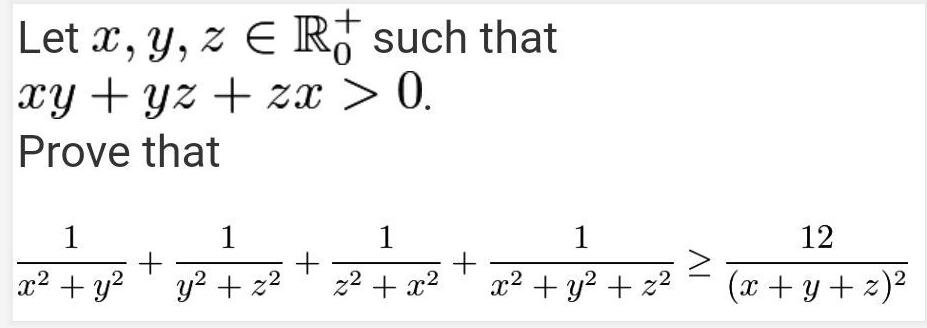
\includegraphics[width=0.6\linewidth]{a010}
\end{center}
\begin{center}
	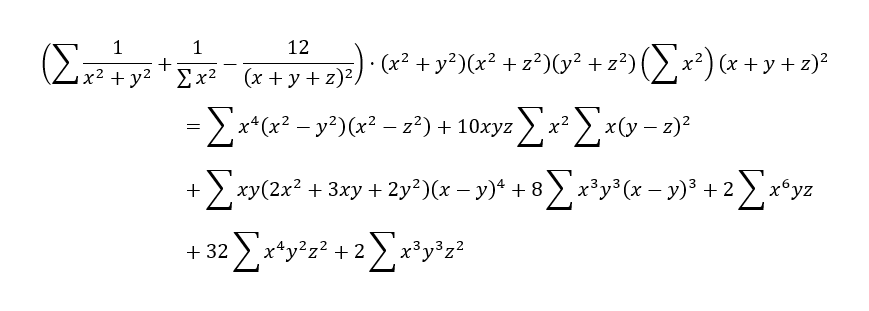
\includegraphics[width=0.7\linewidth]{a020}
\end{center}
通分后的系数是这样
\begin{center}
	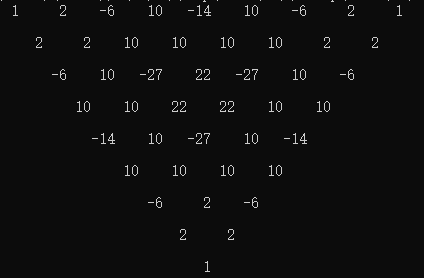
\includegraphics[width=0.7\linewidth]{a030}
\end{center}
注意到$ ab $边上总和为0,所以先schur一下,再在三条边上各自配,中间-27随便搞,我这个配的不是很好看…仔细一看其实上来拿$  \displaystyle \sum a^{6}(a-b)(a-c) $更舒服。其实这里有个小知识点,由于abc=110取等,所以角上这个1要小心用,得保证$ (a,b,c)=(1,1,0) $和$ (1,0,1) $时候都取得到等,为此我们就可以考虑schur了,因为众所周知schur的取等有$ 111,110,101,011 $四个
\begin{center}
	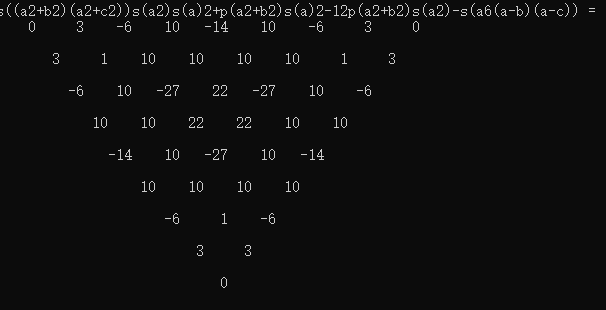
\includegraphics[width=0.7\linewidth]{a040}
\end{center}
那么拿完$  \displaystyle \sum a^{6}(a-b)(a-c) $ 之后是这样,三条边上刚好是$ [3,-6,3][7,-14,7][3,-6,3] $合起来,中间$ -27 $真的就随便搞了
\begin{center}
	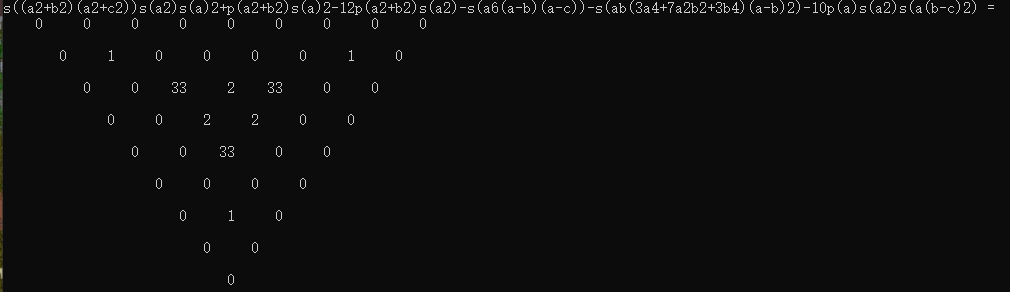
\includegraphics[width=0.7\linewidth]{a050}
\end{center}
\end{document}

(下面是常用的东西,可以先复制到另一个tex方便复制)
代码里搜这些星常用的符号可以快速替换:(ps:不复制这个容易被你自己替换掉)
² $ ^{2} $
³ $ ^{3} $
⁴ $ ^{4} $
Σ $ \displaystyle \sum  $
≥ $ \geq  $
$ 
> < 
\Leftrightarrow 
\Box 
$
链接
\href{https://www.baidu.com/}{这是百度的链接}
系数阵专用
(如果要行内的不复制首尾行即可)
2
\renewcommand*{\arraystretch}{1.732}\[
\left[\begin{matrix}
	1& &1 \\
	& 1&\\
\end{matrix}\right]
\]
3
\renewcommand*{\arraystretch}{1.732}\[
\left[\begin{matrix}
	0& &0& &0\\
	&0& &0&\\
	& &0& &\\
\end{matrix}\right]
\]
4
\renewcommand*{\arraystretch}{1.732}\[
\left[\begin{matrix}
	0& &0& &0& &0\\
	&0& &0& &0&\\
	& &0& &0& & \\
	& & &0& & &\\
\end{matrix}\right]
\]
5
\renewcommand*{\arraystretch}{1.732}\[
\left[\begin{matrix}
	0& &0& &0& &0& &0\\
	&0& &0& &0& &0&\\
	& &0& &0& &0& &\\
	& & &0& &0& & &\\
	& & & &0& & & &\\
\end{matrix}\right]
\]
6
\renewcommand*{\arraystretch}{1.732}\[
\left[\begin{matrix}
	\begin{tabular}{ccccccccccccc}
		0& &0& &0& &0& &0& &0\\
		&0& &0& &0& &0& &0&\\
		& &0& &0& &0& &0& &\\
		& & &0& &0& &0& & &\\
		& & & &0& &0& & & &\\
		& & & & &0& & & & &\\
	\end{tabular}
\end{matrix}\right]
\]
7
\renewcommand*{\arraystretch}{1.732}\[
\left[\begin{matrix}
	\begin{tabular}{ccccccccccccc}
		0& &0& &0& &0& &0& &0& &0\\
		&0& &0& &0& &0& &0& &0&\\
		& &0& &0& &0& &0& &0& &\\
		& & &0& &0& &0& &0& & &\\
		& & & &0& &0& &0& & & &\\
		& & & & &0& &0& & & & &\\
		& & & & & &0& & & & & &\\
	\end{tabular}
\end{matrix}\right]
\]
8
\renewcommand*{\arraystretch}{1.732}\[
\left[\begin{matrix}
	\begin{tabular}{ccccccccccccccc}
		0& &0& &0& &0& &0& &0& &0& &0\\
		&0& &0& &0& &0& &0& &0& &0&\\
		& &0& &0& &0& &0& &0& &0& &\\
		& & &0& &0& &0& &0& &0& & &\\
		& & & &0& &0& &0& &0& & & &\\
		& & & & &0& &0& &0& & & & &\\
		& & & & & &0& &0& & & & & &\\
		& & & & & & &0& & & & & & &\\
	\end{tabular}
\end{matrix}\right]
\]